\subsubsection{فعالیت بالا رفتن از جعبه}

فعالیت بالا رفتن از جعبه یکی از فعالیت‌هایی است که می‌تواند اطلاعات مهمی درباره قدرت اندام‌های تحتانی، توانایی انتقال وزن، کنترل تعادل و هماهنگی حرکتی فراهم کند. در افراد مبتلا به ضعف عضلانی، اجرای این فعالیت ممکن است با کاهش توان بالا بردن بدن، افزایش زمان اجرا، استفاده بیشتر از اندام‌های فوقانی، ناپایداری در انتقال وزن یا به‌کارگیری الگوهای جبرانی همراه باشد. بنابراین، بررسی این فعالیت می‌تواند اطلاعات مفیدی درباره تفاوت میان سطوح عملکردی شبیه‌سازی‌شده فراهم کند و توانایی سامانه در تحلیل فعالیت‌های نیازمند غلبه بر ارتفاع را مورد ارزیابی قرار دهد. داده‌های بررسی‌شده در این بخش مربوط به حالتی هستند که حرکت با قرار دادن پای راست روی جعبه آغاز شده است.

\paragraph{گزارش کلی فعالیت}

در فعالیت بالا رفتن از جعبه با پای راست، حرکت اصلی شامل قرار دادن پای راست روی سطح جعبه، انتقال وزن بدن به این پا، بالا کشیدن بدن و سپس قرار گرفتن پای دیگر روی جعبه است. به همین دلیل، انتظار می‌رود حسگر نصب‌شده روی پای راست نقش مهمی در ثبت شروع حرکت، تغییر زاویه اندام و مرحله انتقال وزن داشته باشد. حسگر پای چپ نیز حرکت پای دنبال‌کننده و تکمیل مرحله بالا رفتن را ثبت می‌کند.

نمونه سیگنال در
\autoref{fig:Climb_Box_Right_Foot_normal_signal_sample}
نشان می‌دهد که علاوه بر حسگرهای نصب‌شده روی پاها، حسگر پیشانی و حسگرهای دست نیز می‌توانند اطلاعاتی درباره کنترل تنه، حفظ تعادل و حرکات جبرانی بدن فراهم کنند. برای مثال، افزایش حرکت دست‌ها ممکن است نشان‌دهنده تلاش فرد برای حفظ تعادل باشد و تغییرات ثبت‌شده توسط حسگر پیشانی می‌تواند نحوه جابه‌جایی تنه در هنگام بالا کشیدن بدن را نشان دهد.

\begin{figure}[H]
	\centering
	
\includegraphics[width=0.80\linewidth]{Images/Generated/TaskResults/Climb_Box_Right_Foot/Normal/signal_sample.png}
	\caption{نمونه سیگنال‌های ثبت‌شده در فعالیت بالا رفتن از جعبه با پای راست}
	\label{fig:Climb_Box_Right_Foot_normal_signal_sample}
\end{figure}

پس از بررسی نمونه سیگنال، سایر مراحل تحلیل مشابه فعالیت ایستادن انجام شد. با توجه به وجود بازه‌های مشخص پیش و پس از اجرای حرکت، اثر جداسازی بازه فعالیت نیز بررسی گردید. نتیجه این مقایسه در
\autoref{fig:climbboxrightfootaccuracybaselinevsdetected}
ارائه شده است. دقت به‌دست‌آمده در حالت جداسازی فعالیت کاهش محسوسی نسبت به حالت بدون جداسازی داشت؛ بنابراین، ادامه روند تحلیل با داده‌های معمولی و بدون جداسازی فعالیت انجام شد.

\begin{figure}[H]
	\centering
	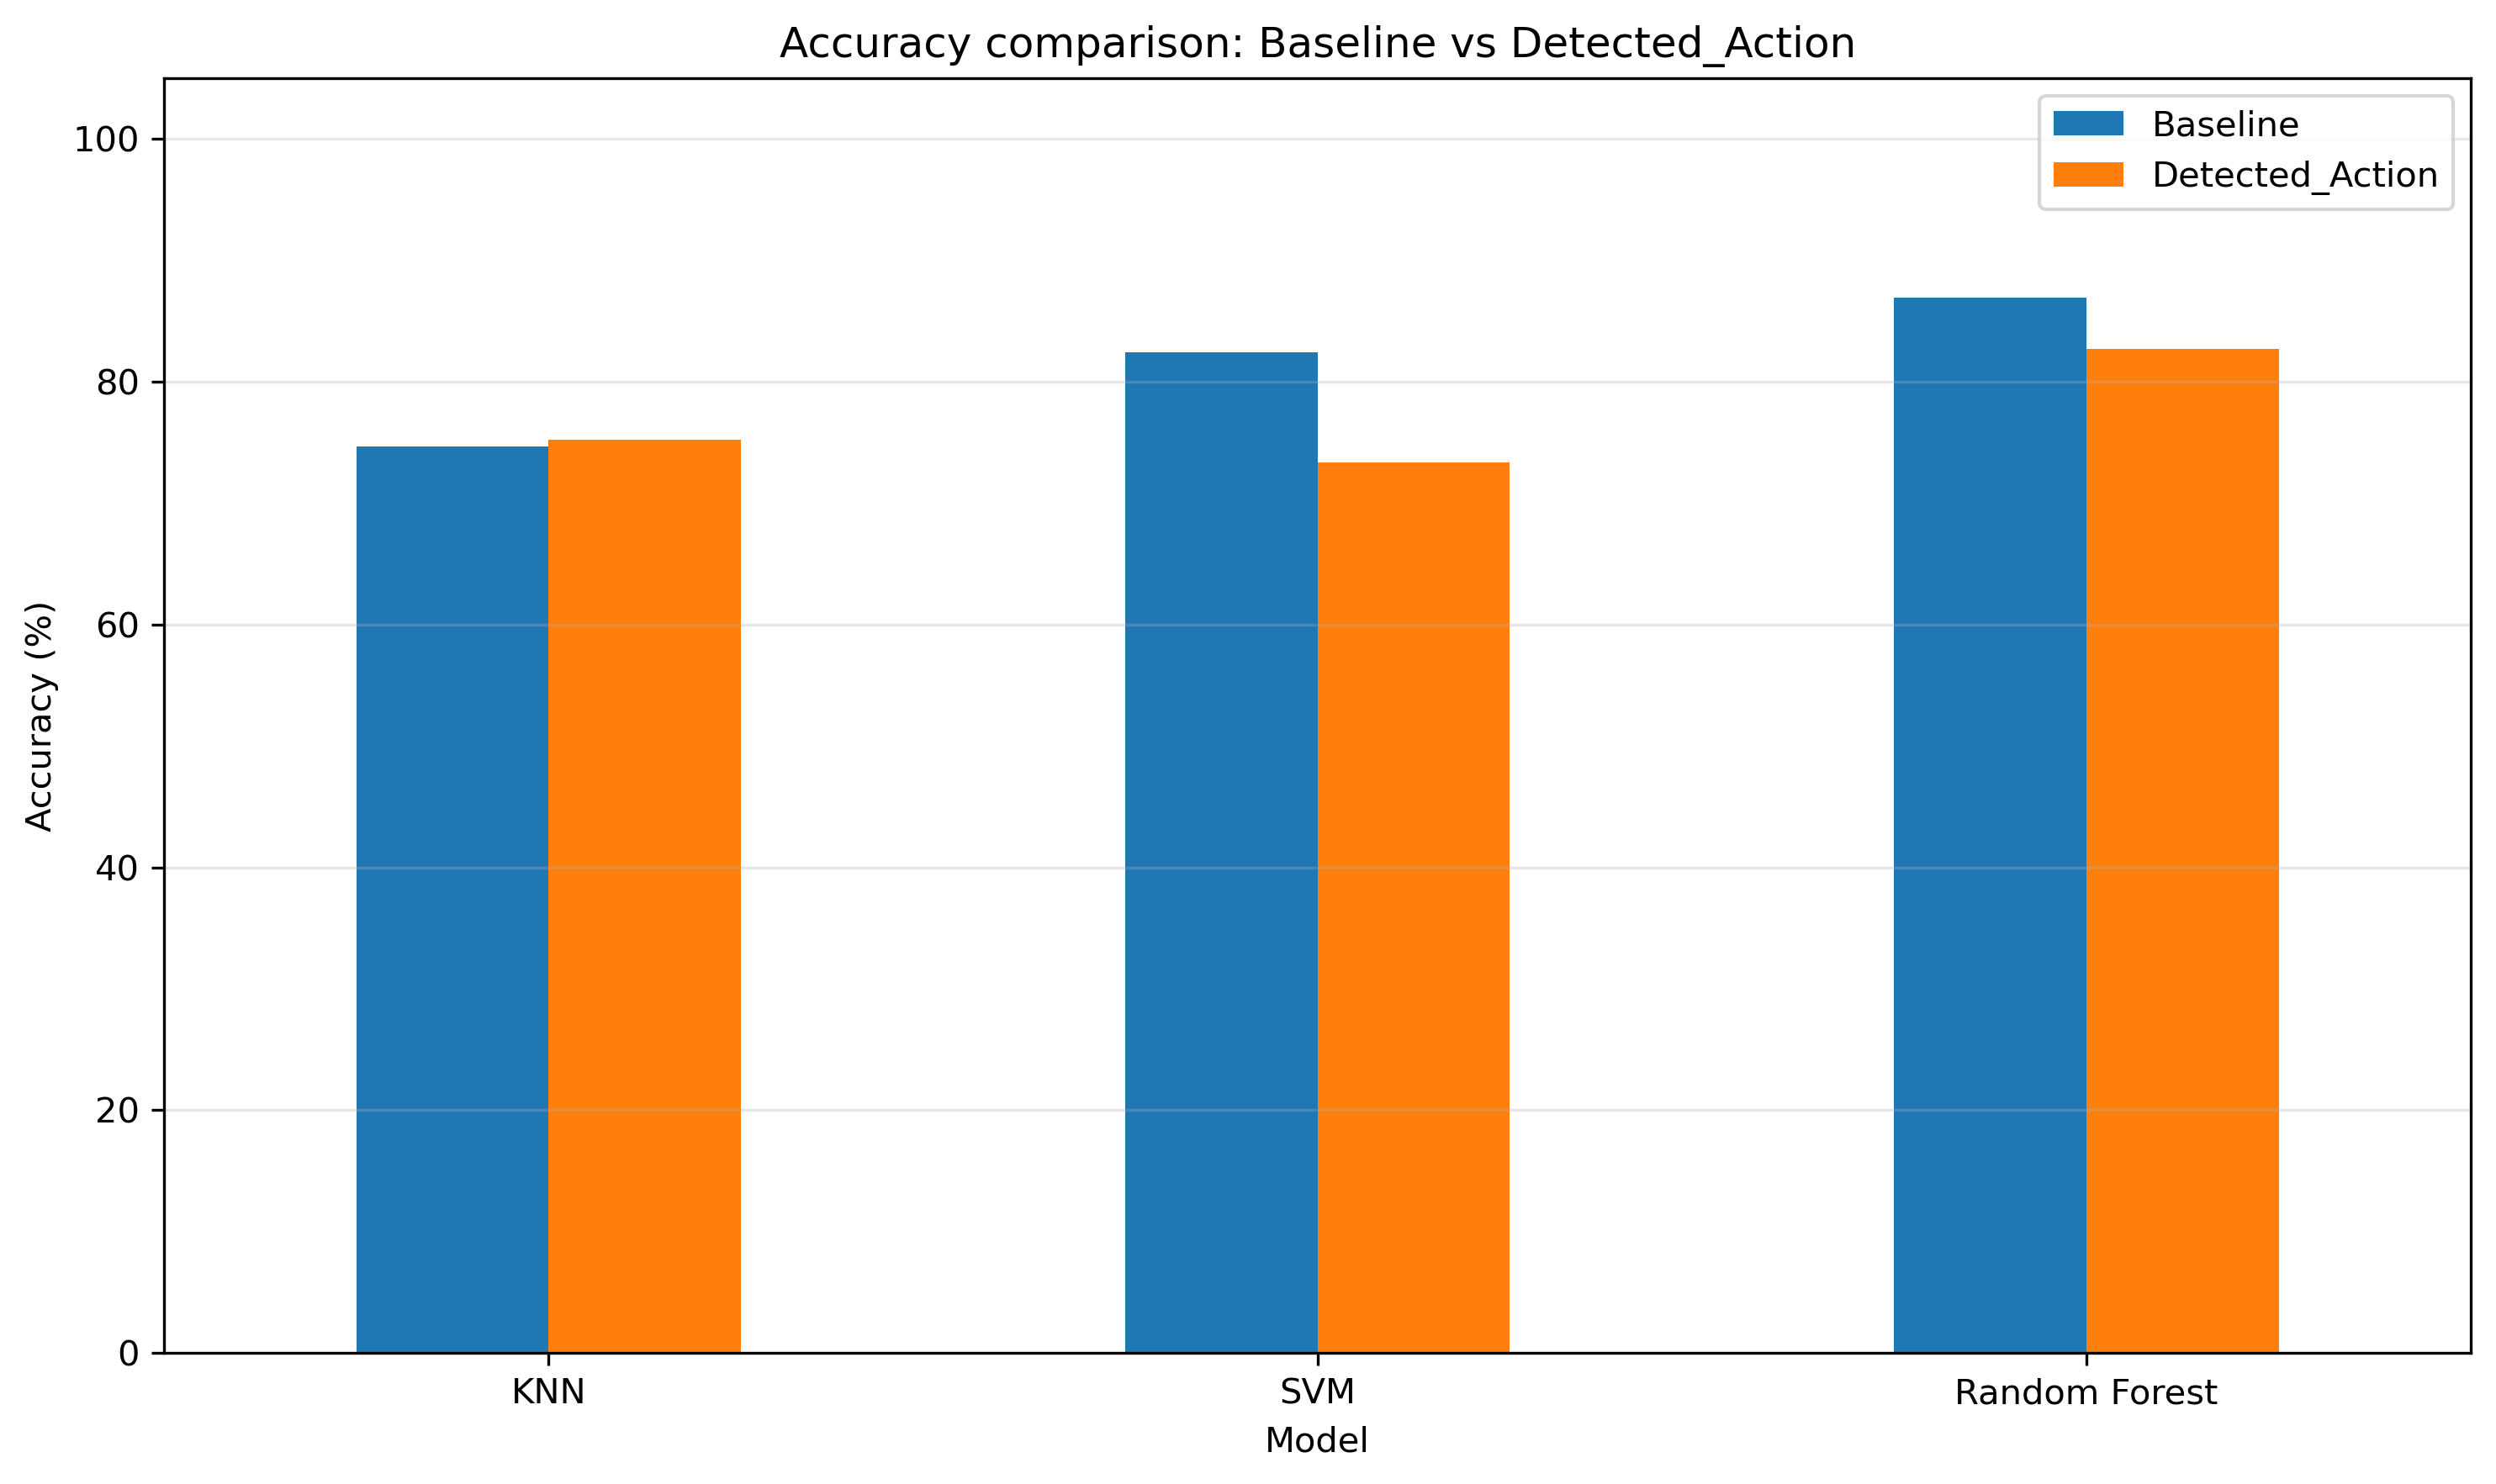
\includegraphics[width=0.7\linewidth]{../Results/Climb_Box_Right_Foot/Comparisons/Accuracy_Baseline_vs_Detected_Action}
	\caption{بررسی اثر جداسازی فعالیت در بالا رفتن از جعبه با پای راست}
	\label{fig:climbboxrightfootaccuracybaselinevsdetected}
\end{figure}

\paragraph{اهمیت ویژگی‌ها و انتخاب مؤلفه‌ها}

اثر تعداد مؤلفه‌های اصلی بر عملکرد مدل منتخب در
\autoref{fig:Climb_Box_Right_Foot_all_metrics_vs_pca}
ارائه شده است. بر اساس این نمودار، با افزایش تعداد مؤلفه‌های اصلی، عملکرد مدل در ابتدا بهبود پیدا می‌کند؛ اما پس از حدود ۱۵ مؤلفه، افزودن مؤلفه‌های جدید لزوماً باعث افزایش قابل‌توجه معیارهای ارزیابی نمی‌شود. این موضوع نشان می‌دهد که بخش اصلی اطلاعات مورد نیاز برای تفکیک سطوح عملکردی در تعداد محدودی از مؤلفه‌ها قرار دارد و استفاده از تمام مؤلفه‌ها برای آموزش مدل ضروری نیست.

\begin{figure}[H]
	\centering
	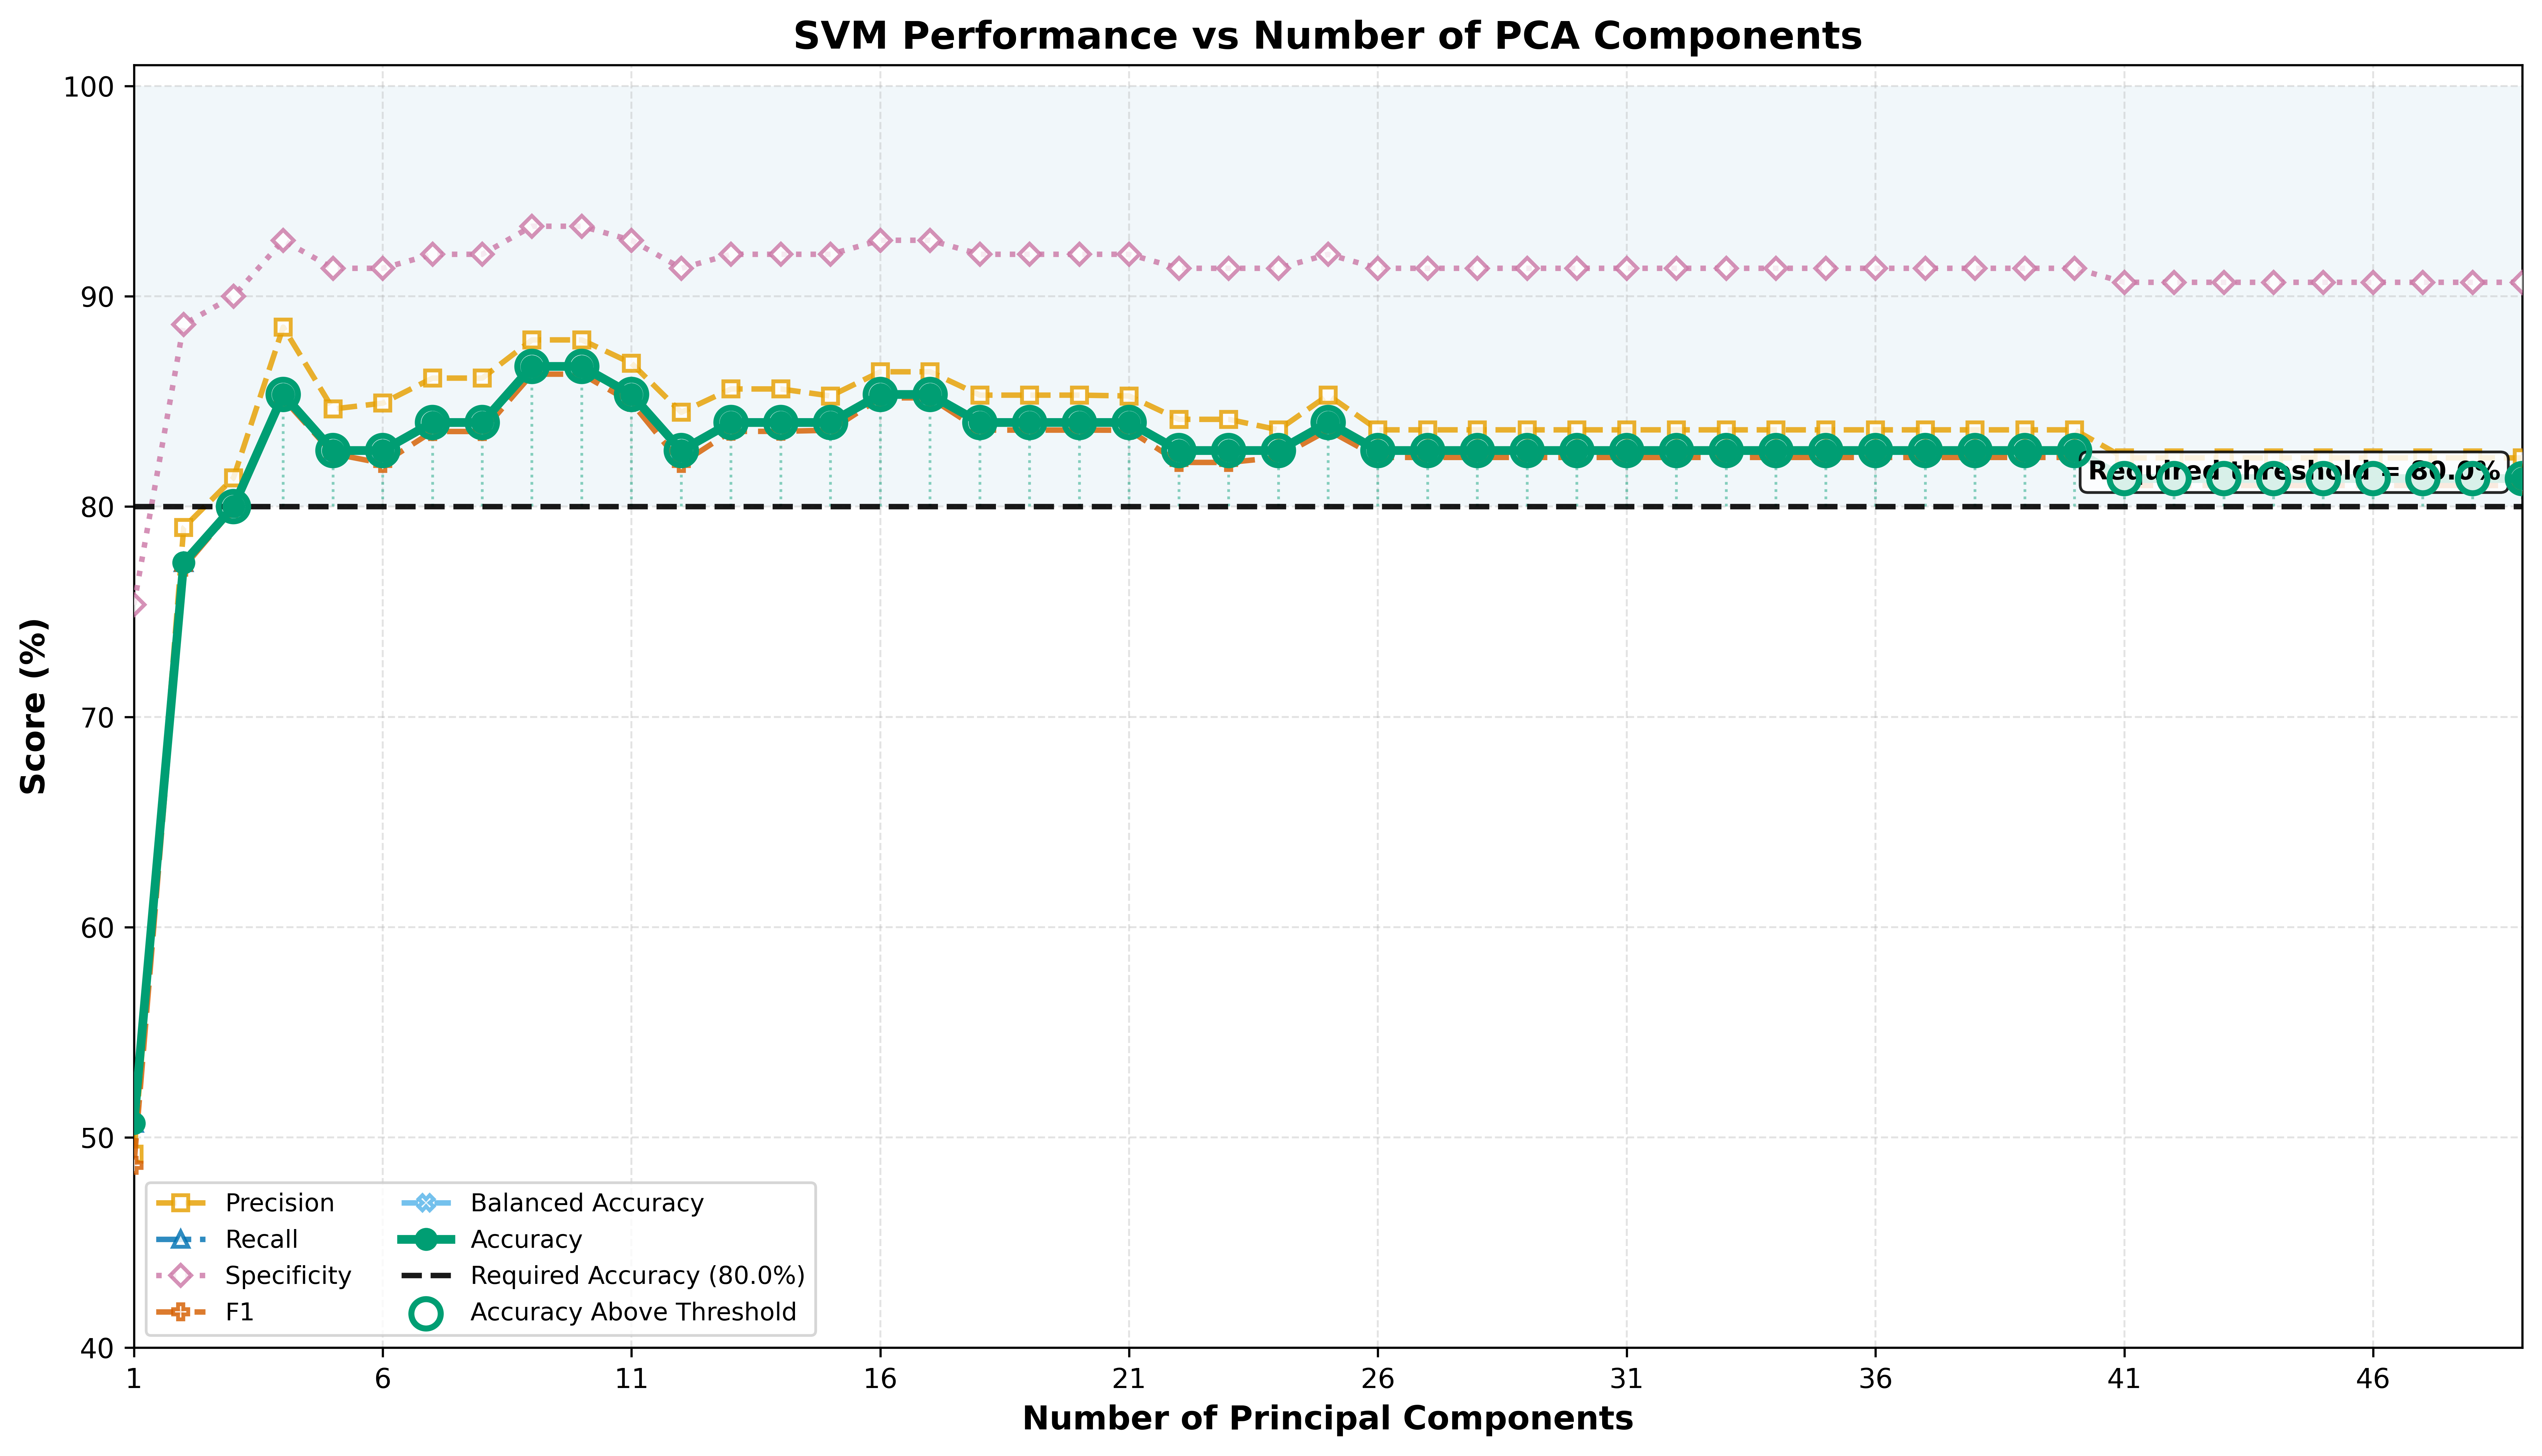
\includegraphics[width=0.8\linewidth]{../Results/Climb_Box_Right_Foot/Normal/FindPrincipalComponents_PipelinePCA_Climb_Box_Right_Foot/Figures/All_Metrics_vs_PCA}
	\caption{تغییر عملکرد مدل منتخب نسبت به تعداد مؤلفه‌های اصلی در فعالیت بالا رفتن از جعبه با پای راست}
	\label{fig:Climb_Box_Right_Foot_all_metrics_vs_pca}
\end{figure}

در نهایت، بر اساس نمودار
\autoref{fig:Climb_Box_Right_Foot_all_metrics_vs_pca}،
مدل‌ها در بازه ۵ تا ۱۵ مؤلفه اصلی دوباره مقایسه شدند تا مدل برتر و تعداد مؤلفه‌های اصلی بهینه تعیین شود. بر اساس نتایج به‌دست‌آمده در
\autoref{fig:Climb_Box_Right_Foot_models_vs_pca_components}،
برای فعالیت بالا رفتن از جعبه با پای راست، مدل ماشین بردار پشتیبان با ۱۰ مؤلفه اصلی انتخاب شد. این ترکیب، ضمن کاهش قابل‌توجه تعداد ابعاد ورودی، دقتی بالاتر از حد نصاب ۸۰ درصد فراهم کرد. بنابراین، افزایش تعداد مؤلفه‌ها بیش از این مقدار، با توجه به افزایش پیچیدگی مدل، بهبود کافی و متناسبی در عملکرد ایجاد نمی‌کرد.

\begin{figure}[H]
	\centering
	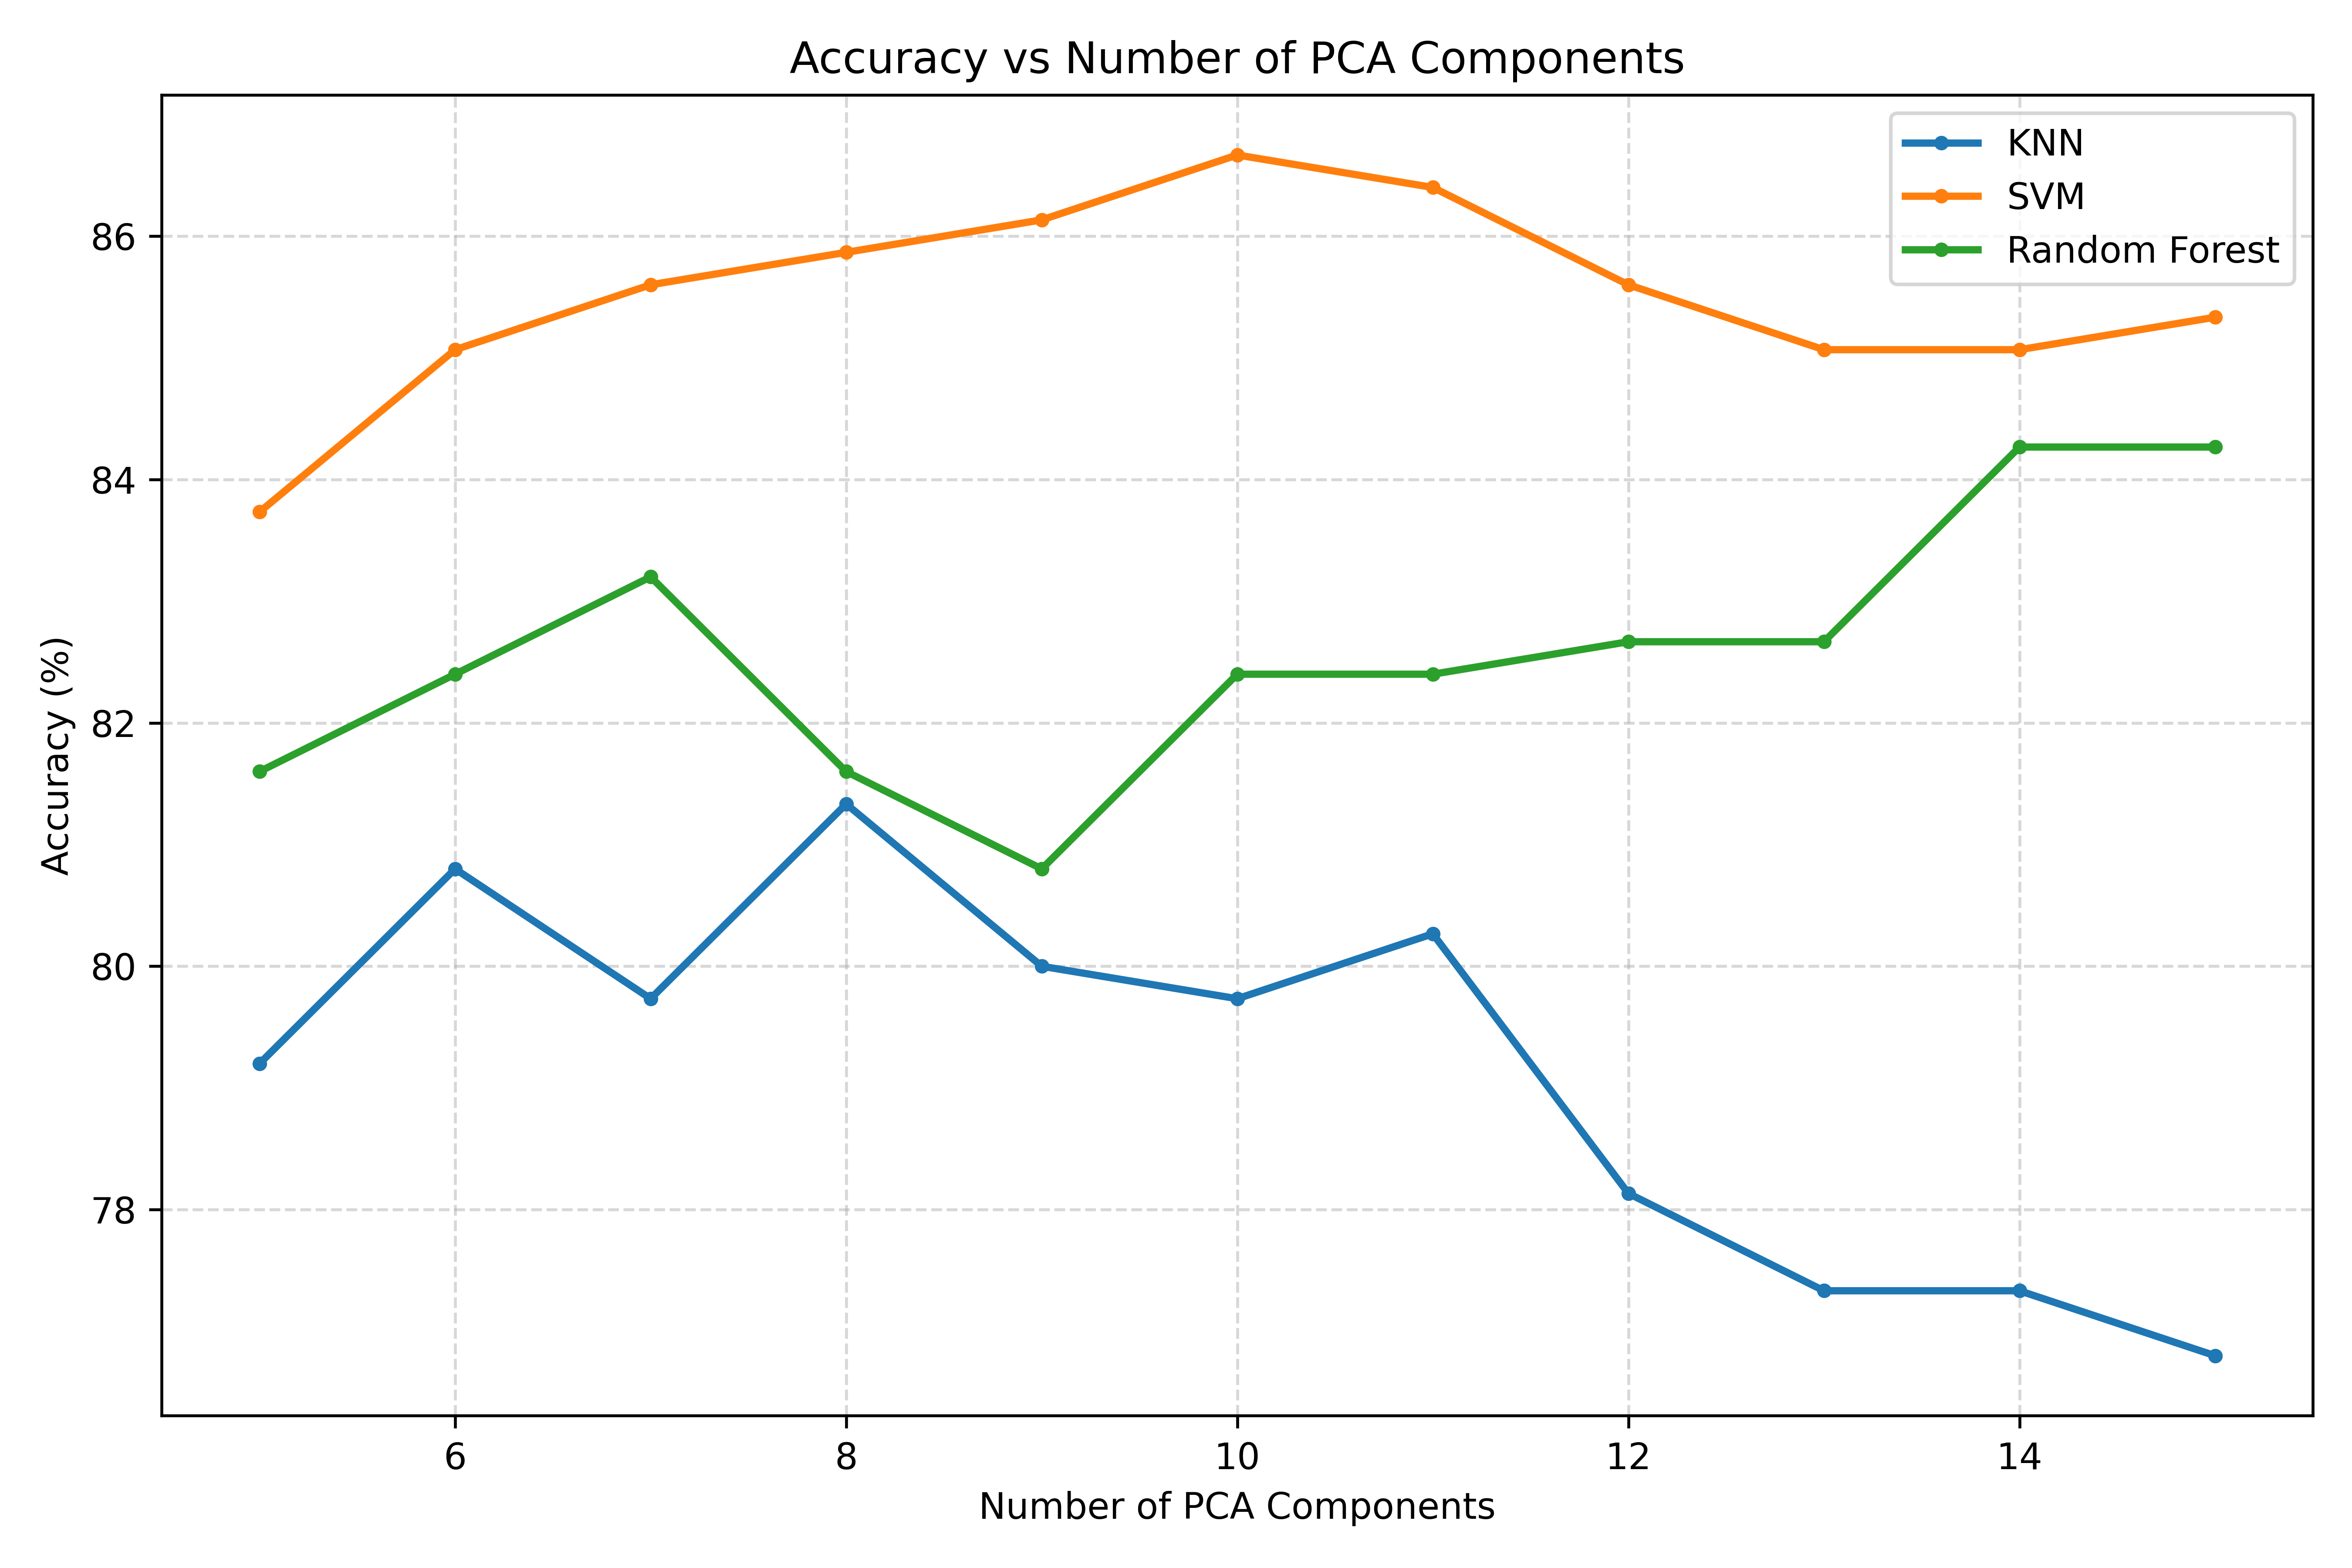
\includegraphics[width=0.8\linewidth]{../Results/Climb_Box_Right_Foot/Normal/CompareNumberOfPrincipalComponents_PipelinePCA_Climb_Box_Right_Foot/Figures/Accuracy_vs_PCA_Components}
	\caption{تغییر دقت مدل‌ها نسبت به تعداد مؤلفه‌های اصلی در فعالیت بالا رفتن از جعبه با پای راست}
	\label{fig:Climb_Box_Right_Foot_models_vs_pca_components}
\end{figure}

\begin{table}[H]
	\centering
	\caption{تنظیمات منتخب فعالیت بالا رفتن از جعبه با پای راست برای مدل نهایی}
	\label{tab:Climb_Box_Right_Foot_selected_setup}
	\begin{tabular}{lcccc}
		\toprule
		نوع داده & مدل منتخب & تعداد مؤلفه اصلی & معیار ارزیابی & حد نصاب معیار \\
		\midrule
		بدون جداسازی فعالیت & ماشین بردار پشتیبان & ۱۰ & دقت & ۸۰ درصد \\
		\bottomrule
	\end{tabular}
\end{table}

\paragraph{جمع‌بندی فعالیت بالا رفتن از جعبه با پای راست}

در فعالیت بالا رفتن از جعبه با پای راست، مدل منتخب معرفی‌شده در
\autoref{tab:Climb_Box_Right_Foot_selected_setup}
با استفاده از اعتبارسنجی متقاطع طبقه‌بندی‌شده مورد ارزیابی قرار گرفت. نتایج نشان می‌دهند که ویژگی‌های حرکتی استخراج‌شده از حسگرها، به‌ویژه حسگرهای نصب‌شده روی پاها، قابلیت استفاده برای تفکیک سه سطح عملکردی شبیه‌سازی‌شده این فعالیت را دارند.

مدل ماشین بردار پشتیبان با استفاده از ۱۰ مؤلفه اصلی به‌عنوان مدل نهایی انتخاب شد. مؤلفه‌های اصلی منتخب حدود ۶۵ درصد از واریانس داده‌های اولیه را در بر می‌گیرند. این نتیجه نشان می‌دهد که برای دستیابی به عملکرد مناسب مدل، حفظ تمام واریانس داده‌ها ضروری نبوده و اطلاعات مؤثر مربوط به انتقال وزن، بالا کشیدن بدن و حفظ تعادل در تعداد محدودی از مؤلفه‌ها خلاصه شده‌اند.

در این ارزیابی، داده‌ها در هر مرحله به ۵ بخش تقسیم شدند و فرایند اعتبارسنجی ۵ مرتبه تکرار شد. نتایج حاصل از تقسیم‌بندی‌های مختلف در
\autoref{fig:Climb_Box_Right_Foot_cv_fold_metrics}
ارائه شده‌اند. بررسی نتایج تقسیم‌بندی‌های مختلف امکان ارزیابی میزان ثبات مدل و وابستگی عملکرد آن به نحوه انتخاب داده‌های آموزش و آزمون را فراهم می‌کند.

\begin{figure}[H]
	\centering
	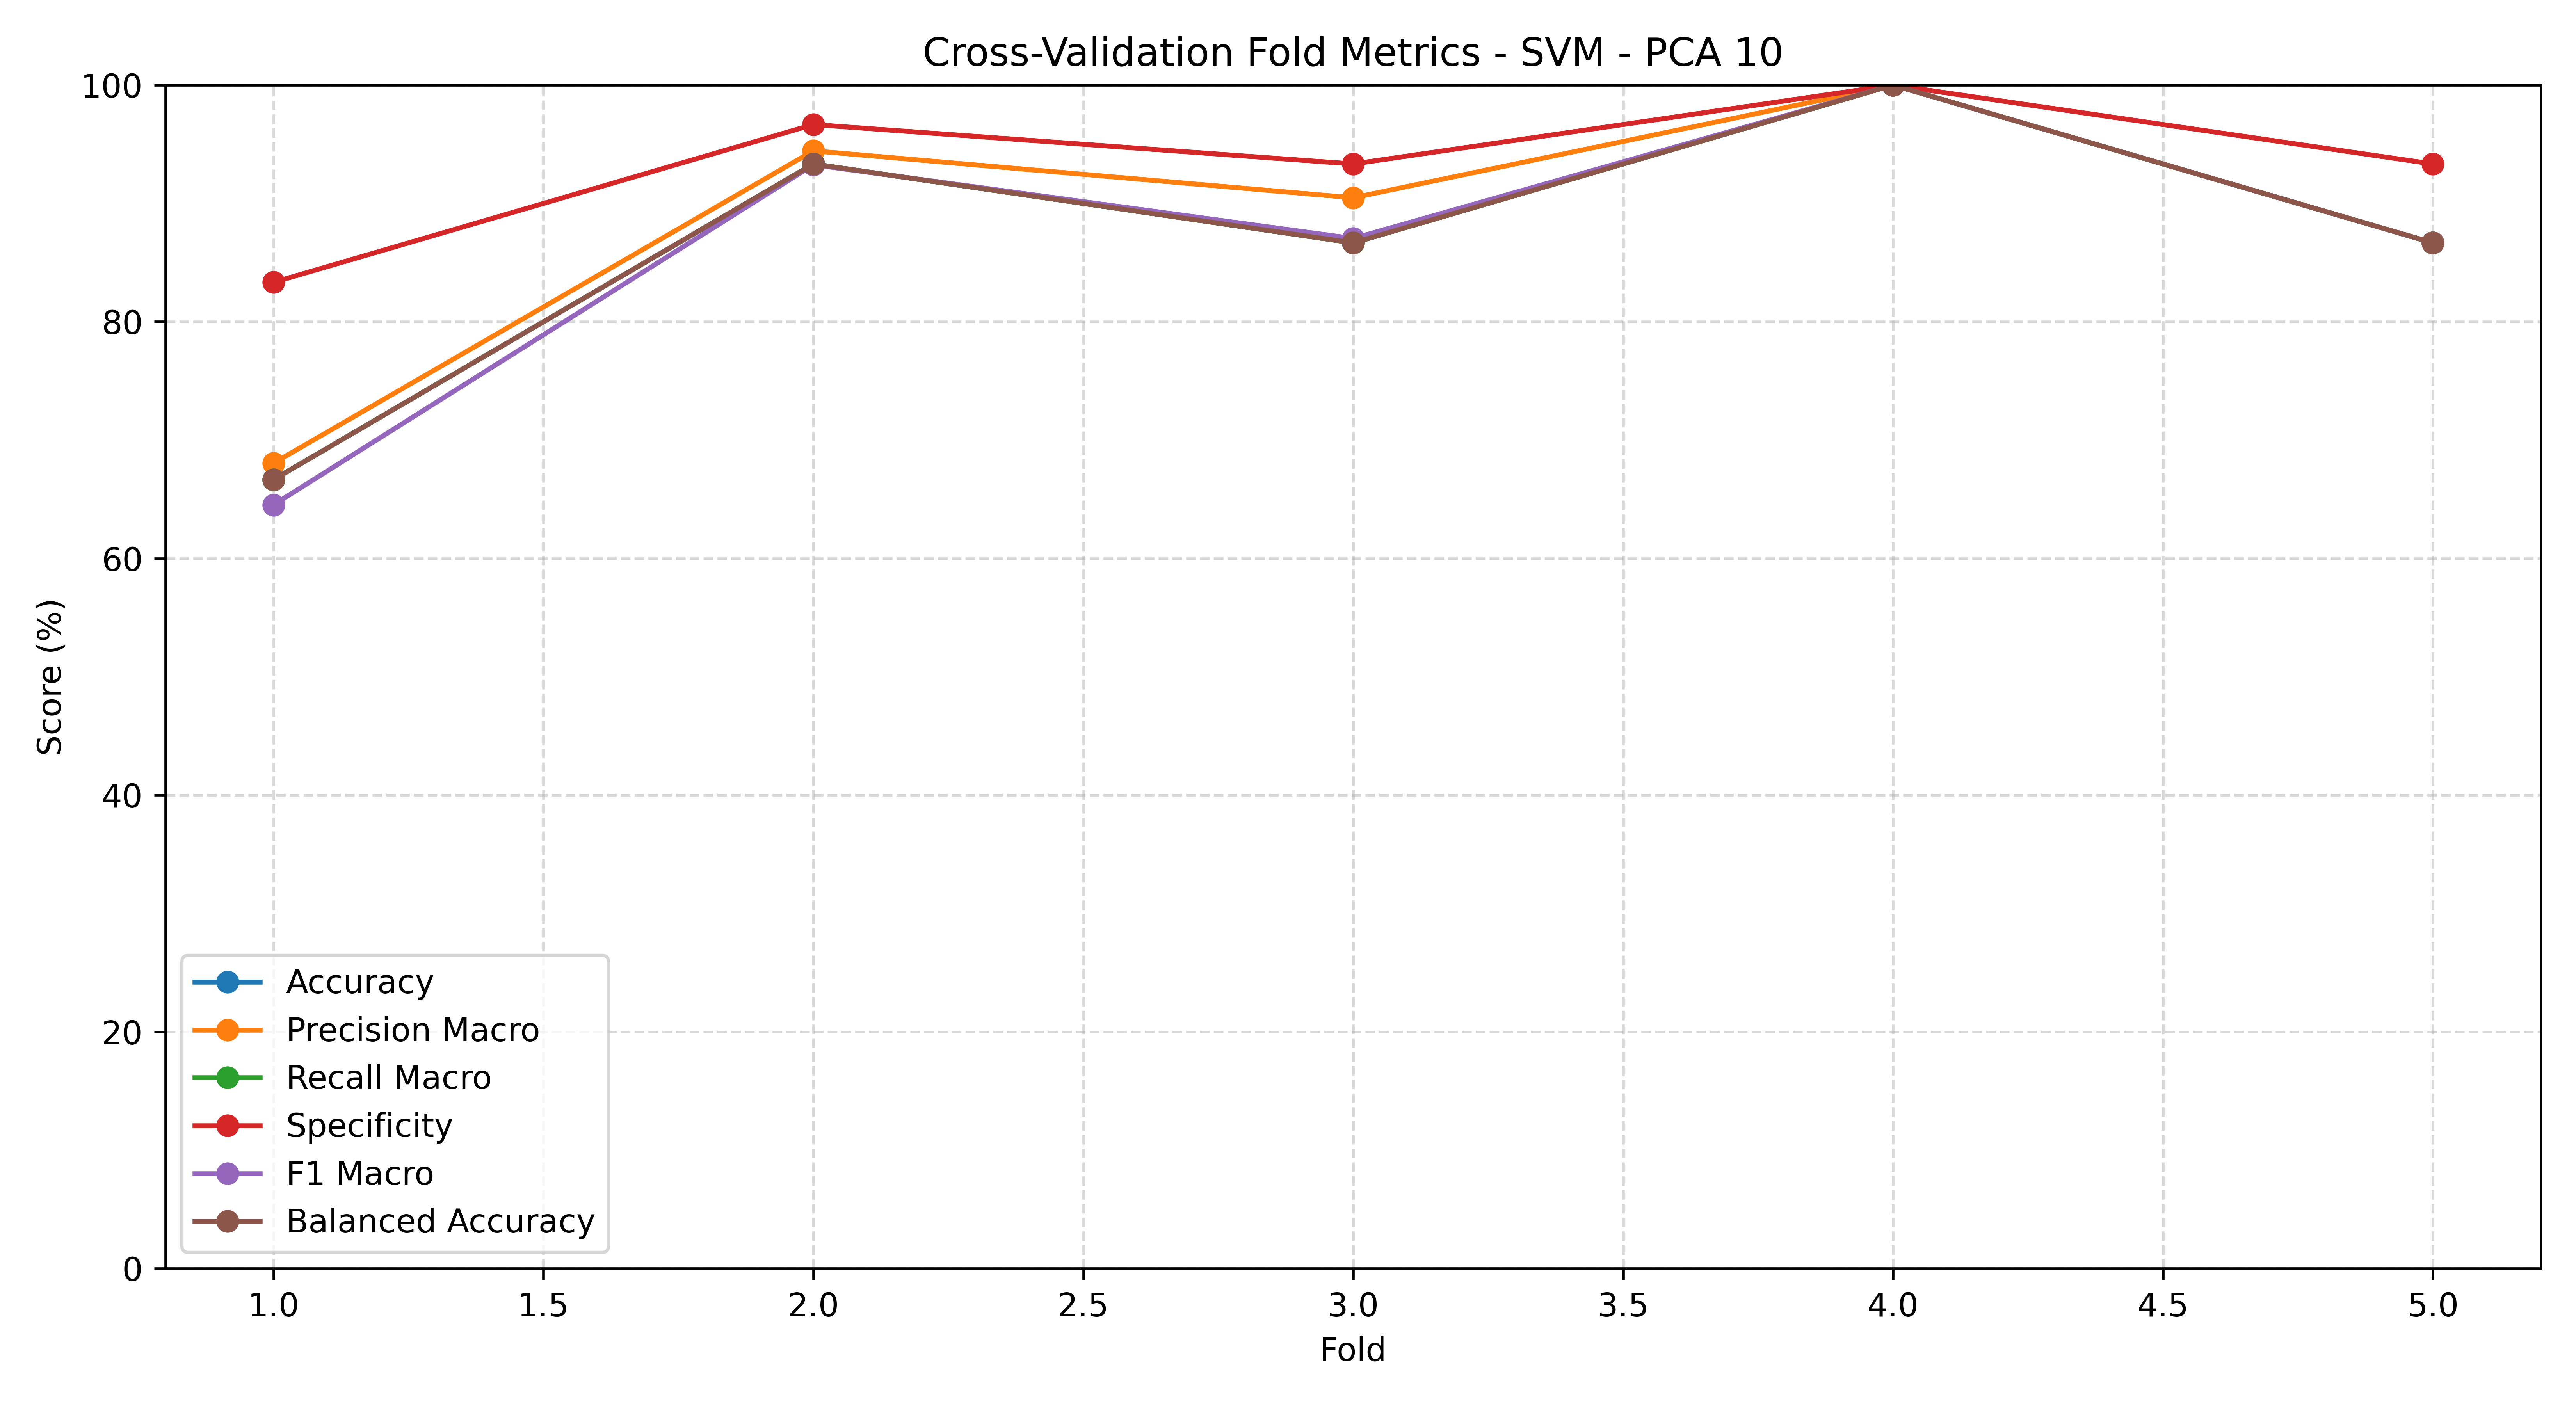
\includegraphics[width=0.8\linewidth]{../Results/Climb_Box_Right_Foot/Final/Final_Model_SVM_PCA10/Figures/CV_Fold_Metrics}
	\caption{نتایج ارزیابی مدل منتخب برای فعالیت بالا رفتن از جعبه با پای راست در تقسیم‌بندی‌های مختلف}
	\label{fig:Climb_Box_Right_Foot_cv_fold_metrics}
\end{figure}

در مجموع، نتایج این فعالیت نشان می‌دهند که تحلیل اطلاعات حسگرهای نصب‌شده روی پاها می‌تواند تغییرات مربوط به شروع حرکت، انتقال وزن و بالا کشیدن بدن را آشکار کند. حسگر پیشانی نیز اطلاعاتی درباره حرکت تنه و کنترل وضعیت بدن ارائه می‌دهد و حسگرهای دست می‌توانند برای شناسایی حرکات جبرانی و تلاش برای حفظ تعادل مورد استفاده قرار گیرند. از آنجا که اجرای بررسی‌شده با پای راست آغاز شده است، نقش حسگر پای راست در توصیف مرحله اصلی انتقال وزن و صعود اهمیت ویژه‌ای دارد.
